%%% Local Variables:
%%% TeX-command-extra-options: "-shell-escape"
%%% mode: latex
%%% TeX-master: t
%%% End:
\documentclass{beamer}
\usepackage{caption}
\usepackage{minted}
\usepackage{tikz}
\usepackage{xcolor}
\usetikzlibrary{shapes.geometric, arrows}
\tikzstyle{startstop} = [rectangle, rounded corners, minimum width=3cm, minimum height=1cm,text centered, draw=black, fill=red!30]
\tikzstyle{io} = [trapezium, trapezium left angle=70, trapezium right angle=110, minimum width=1.5cm, minimum height=0.6cm, text centered, draw=black, fill=blue!30]
\tikzstyle{process} = [rectangle, minimum width=1.5cm, minimum height=0.5cm, text centered, draw=black, fill=orange!30]
\tikzstyle{decision} = [circle, radius=2.5cm, text centered, draw=black, fill=green!30]
\tikzstyle{arrow} = [thick,->,>=stealth]
\usepackage[labelformat=simple]{subcaption}

\usetheme{Singapore}
\title{Arbitrarily Large Data}
\begin{document}
\begin{frame}
\titlepage
\end{frame}
\section{Lists}

\begin{frame}
  \huge \emph{Recursion} - see recursion
\end{frame}

\begin{frame}
  \frametitle{Self Referentiality Powerful and Scary}
  \begin{figure}
    \begin{subfigure}{0.3\textwidth}
      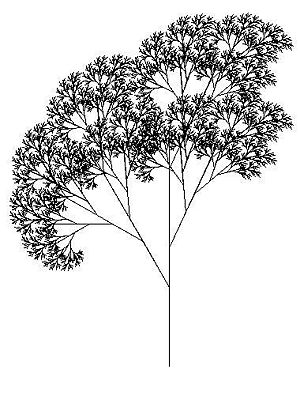
\includegraphics[width=0.9\textwidth]{images/recursive-tree.JPG}
    \end{subfigure}
    \begin{subfigure}{0.3\textwidth}
      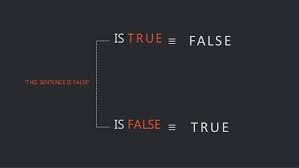
\includegraphics[width=0.9\textwidth]{images/liars-paradox.jpeg}
    \end{subfigure}
    \begin{subfigure}{0.3\textwidth}
      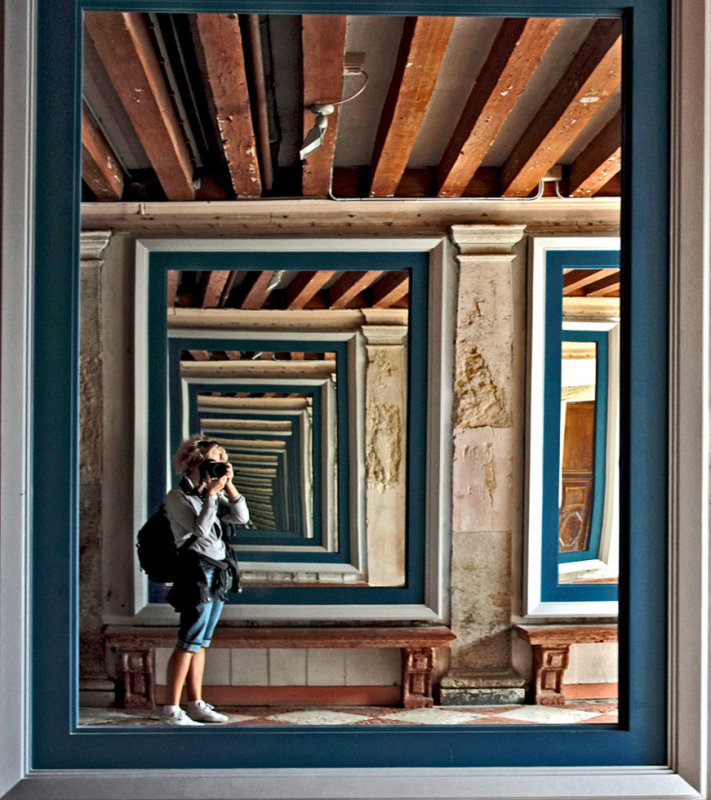
\includegraphics[width=0.9\textwidth]{images/reflections.jpg}
    \end{subfigure}
  \end{figure}
\end{frame}

\begin{frame}
  \frametitle{Self Referentiality}
  The ability to self reference is \emph{powerful} but also \emph{troublesome}.
  \begin{itemize}
  \item<2-> Through self referentiality, we can construct the most basic mathematical tool that has
    been proven to be a powerful concept throughout history--the natural numbers.
  \item<3-> This leads to many other powerful structures like other numbers, lists, trees, etc.
  \item<4-> But we also got the first instances of extremely troublesome concepts--paradoxes.
  \item<5-> The omnipotence paradox - asked if it was possible for a being to exist so powerful that it could create a stone that it could not lift.
  \item<6-> The Epimenides paradox, 'All Cretans are liars' when uttered by an ancient Greek Cretan was one of the first recorded versions. 
  \end{itemize}
\end{frame}

\begin{frame}
  \frametitle{Self Referential Data and Racket}
  So far, we have only written programs with fixed size data (well numbers and strings aren't truly fixed size but they are primitive).
  \begin{itemize}
  \item<2-> We don't currently have a way to specify data definitions for extensible data.
  \item<3-> Consequently, we can't support the creation of programs like a space invaders game with
    flexible numbers of enemies.
  \item<4-> So we will change how we specify data definitions to support things like this and will revise our design recipes
    for dealing with extensible data
  \end{itemize}
\end{frame}

\begin{frame}
  \frametitle{Lists: A Fundamental Structure }
  One of the most important things to get used to in functional programming is dealing with lists.
  \begin{itemize}
  \item<2-> Lists are quite common in programming in general as a way to store related data for processing data.
  \item<3-> A large part of the execution time of many programs is spent iterating over lists.
  \item<4-> The simplest list we can specify is the empty list \mintinline{racket}{'()}
  \item<5-> We can start building lists with \mintinline{racket}{cons}--for example
    \mintinline{racket}{(cons 1 '())} $\hookrightarrow$ \mintinline{racket}{'(1)}.
  \item<6-> We can also use other types like strings in our lists \mintinline{racket}{(cons "Mercury" '())}
  \end{itemize}
\end{frame}

\begin{frame}
  \frametitle{Analyzing Cons Cells}
  Let's consider the following list: \mintinline{racket}{(cons "Mercury" '())}.
  \begin{itemize}
  \item<2-> We have the following visual representation of this list:
    \includegraphics[width=0.2\textwidth]{images/mercury-cons.png}
  \item<3-> For \mintinline{racket}{(cons "Earth" (cons "Venus" (cons "Mercury" '()))))}
    we have the following visual representation:
    \includegraphics[width=0.35\textwidth]{images/planet-cons.png}
  \end{itemize}
\end{frame}

\begin{frame}
  \frametitle{Cons Cell Properties}
  The nested representation of cons cells gets complicated as lists get larger, very quickly.
  \begin{itemize}
  \item<2-> Programmers usually opt to think about them in terms of box and pointer diagrams instead:
    \includegraphics[width=0.5\textwidth]{images/box-pointer-back.png}
  \item<3-> It's more natural to think about this in a more forward manner however, where the box on the
    left corresponds to the \emph{head} of the list and there is a pointer to the \emph{tail} of the list:
    \includegraphics[width=0.5\textwidth]{images/box-pointer-forward.png}
  \end{itemize}
\end{frame}

\begin{frame}
  \frametitle{Some Weird Lists}
  By this point, you may be used to thinking about lists as \emph{homogeneous} collections of items.
  \begin{itemize}
  \item<2-> But you can also creates lists from elements of different types:
    \mintinline{racket}{(cons "Peter" (cons 26 (cons \#t '())))}
  \item<3-> In this list we have a string, an integer, and a boolean value.
  \item<4-> We can also think about adding structs or functions to our list.
  \item<5-> Alternatively, instead of thinking about our list as being unstructured,
    we could say that is a list whose values are an itemization of strings, integers, and true.
  \item<6-> If we cons on a new value with a type not present in the itemization, then we could define
    an itemization that extends our previous one.
  \item<7-> And building on my previous lectures, we can even think of this list as representing
    something like a person. But in that case we should define a struct!
  \end{itemize}
\end{frame}

\defverbatim[colored]\ThreeList{
\begin{minted}[fontsize=\footnotesize]{racket}
    ; A 3LON is a list of three numbers: 
    ;   (cons Number (cons Number (cons Number '())))
    ; interpretation a point in 3-dimensional space 
\end{minted}
}

\begin{frame}
  \frametitle{Data Definitions and Lists}
  Consider the following list: \mintinline{racket}{(cons 1 (cons 2 (cons 3 '())))}
  \begin{itemize}
  \item<2-> What kind of data definition could we given for this list?
  \item<3-> \ThreeList
  \item<4-> Again, such a data definition seems more appropriate for struct.
  \item<5-> More importantly, the list is extensible and this definition
    doesn't address the fact that consing an additional element to
    the aforementioned list creates a value outside of this definition.
  \item<6-> So how do we talk about data definitions
    where we can construct values of arbitrarily large size?
  \end{itemize}
\end{frame}

\defverbatim[colored]\ListOfNames{
\begin{minted}[fontsize=\footnotesize]{racket}
    ; A List-of-names is one of: 
    ; – '()
    ; – (cons String List-of-names)
    ; interpretation a list of guests, by last name
\end{minted}
}

\begin{frame}
  \frametitle{Lists are Recursively Defined}
  Let's say that we are designing a program for hotel booking for a large
  hotel. For a given weekend we need a list of dynamic size for our
  guest list.
  \begin{itemize}
  \item<2-> Assuming we only store the guest's last name, how do we shape
    our data definition to meet this dynamic size requirement?
  \item<3-> \ListOfNames
  \item<4-> Such a definition should seem familiar to you at this point.
  \item<5-> When programming data structures in Java, you should have
    become used to recursive instances of a class in a class definition.
  \end{itemize}
\end{frame}

\begin{frame}
  \frametitle{List-of-names Examples}
  What are some example values of our List-of-names definition?
  \begin{itemize}
  \item<2-> Starting with the first clause of our definition's itemization,
    we have a nice atomic element.
  \item<3-> This element is the empty list \mintinline{racket}{'()} and forms the smallest  value in our list.
  \item<4-> The most simple elements of \emph{inductively} defined data are known
    as our base values, in correspondance with the \emph{base case} of an
    inductive proof.
  \item<5-> Don't worry about this too much for now, let's look
    at more values of our data definition.
  \item<6-> In order to construct a more complicated list, we look at the second clause of our itemization. We must cons a string
    onto another list, but so far we only know how to constuct the empty list.
  \item<7-> This allows us to define a single element list like:
    \mintinline{racket}{(cons "Nadal" '())}
  \end{itemize}
\end{frame}

\begin{frame}
  \frametitle{List-of-names Examples (cont.)}
  How do we create a two element guest list?
  \begin{itemize}
  \item<2-> Easy, we apply the second case of our itemization again and cons something onto a one element list!
  \item<3-> \mintinline{racket}{(cons "Federer" (cons "Nadal" '()))}
  \item<4-> And of course, we can inductively keep constructing an arbitrary
    list of size N+1 from a list of size N.
  \item<5-> This brings an interesting point up. Can I use induction to prove
    things about propositions that are generated from things besides natural numbers?
  \item<6-> Yes, inductively defined types come with their own induction principles. Programming language theorists do induction over different structures often.
  \item<7-> But back to programming land! We seemed to brush over some details.
    What exactly are \mintinline{racket}{'()} and \mintinline{racket}{cons}?
  \end{itemize}
\end{frame}

\section{Atoms and Constructors}
\begin{frame}
  \frametitle{Empty Lists and Cons}
  ...
\end{frame}
\end{document}
%%% Local Variables:
%%% TeX-command-extra-options: "-shell-escape"
%%% mode: latex
%%% TeX-master: t
%%% End:
